\begin{figure}[hbt!]
    \centering
    \begin{tikzpicture}
    \node[anchor=south west,inner sep=0] (image) at (0,0) {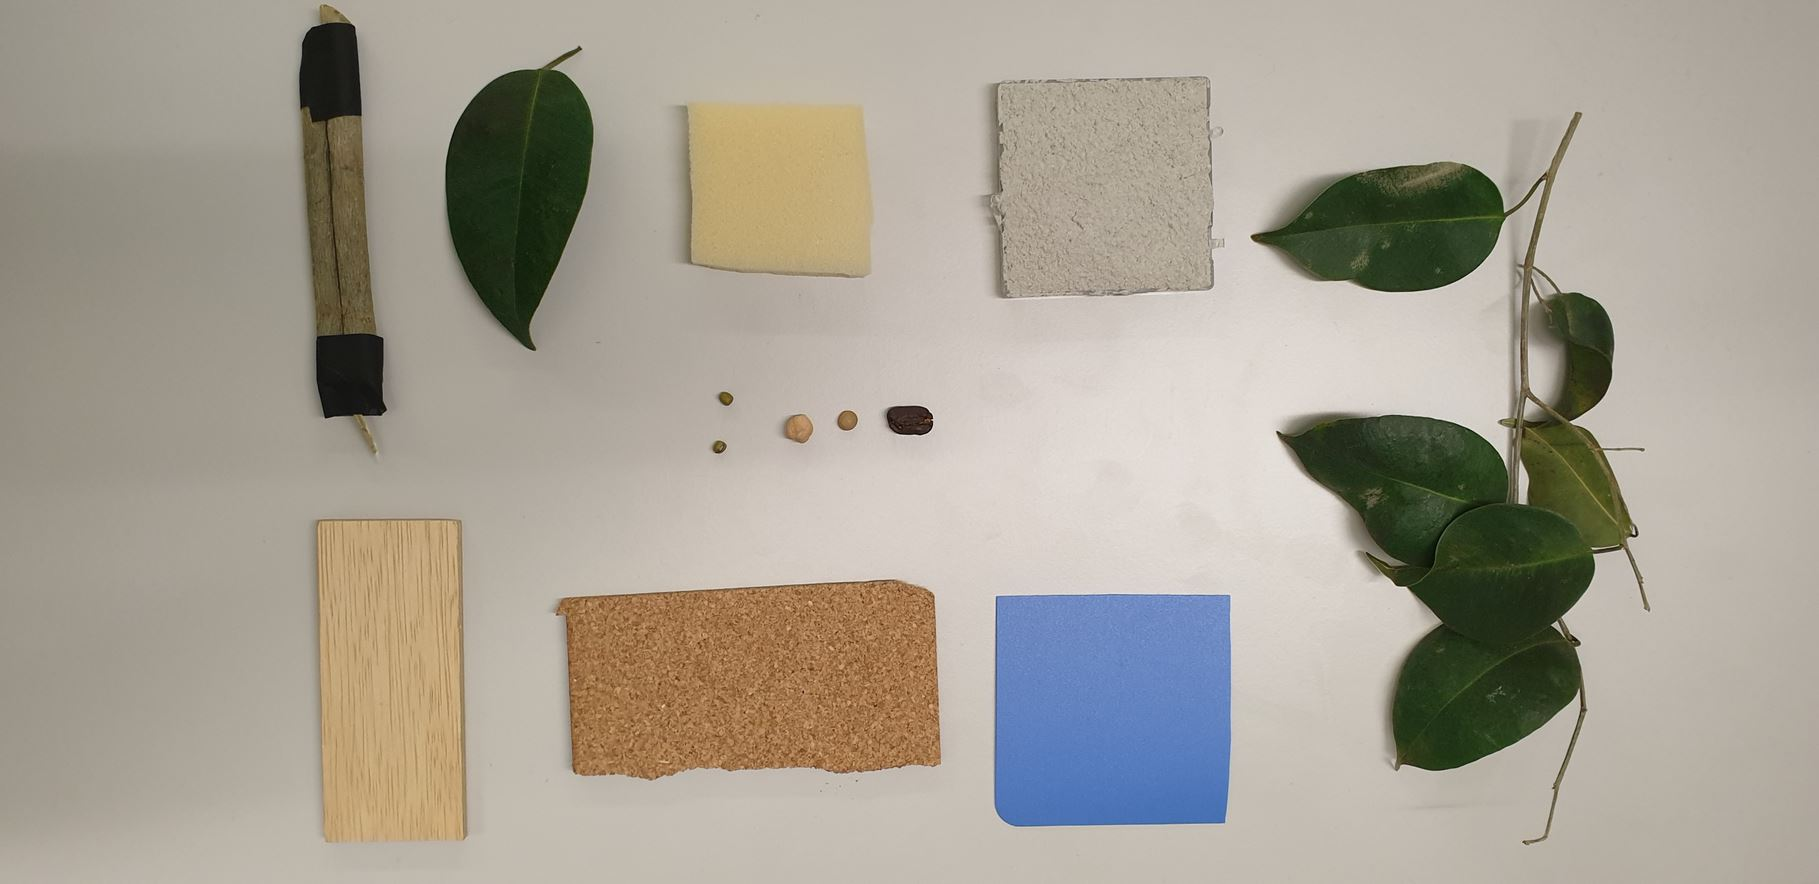
\includegraphics[width=\linewidth]{chapters/papers/ED/resources/images/multi-spectral/material_samples.png}};
    \begin{scope}[x={(image.south east)},y={(image.north west)}]
        \node [rounded corners, fill=white] at (0.18, 0.92) {branch};
        \node [rounded corners, fill=white] at (0.29, 0.92) {leaf};
        \node [rounded corners, fill=white] at (0.42, 0.92) {foam};
        \node [rounded corners, fill=white] at (0.6, 0.92) {plaster};
        \node [rounded corners, fill=white] at (0.21, 0.38) {wood};
        \node [rounded corners, fill=white] at (0.42, 0.38) {cork};
        \node [rounded corners, fill=white] at (0.6, 0.38) {plastic};
    \end{scope}
    \end{tikzpicture}%
\caption{Materials used for evaluating our setup}
\label{fig:materials}
\end{figure}
